\section{Theory}\label{theory}
This section presents background information on digital image processing and one small section explaining light scattering, as this is an important part when dealing with underwater imaging.
There was not found any suggestions from the literature on how to solve the exact problem of underwater depthmap images, but there are many different approaches that solves parts of the problem.
Below follows different methods containing theory and solutions for various types of image enhancement on 2D images. 


\subsection{Filtering in the Spatial Domain}

Filtering is a technique for enhancing or modifying an image, but it can also be used to blur an image. It is used to highlight or remove certain features in an image, or both. Different techniques include smoothing, sharpening and edge enhancement. 
Filtering is a neighborhood operation, meaning that each pixels value is determined by the values of the neighboring pixels. The algorithms run though each pixel in the image and replaces the value with some value determined by the filter matrix. The matrix holding the filter is called the kernel, and the kernel size determines how big the neighborhood of the filtering will be. Filters where the output pixel is a linear combination of the values in the input pixels neighborhood is called linear filters. Averaging filter is an example of a linear filter.\cite{book:digital_image_processing}\cite{website:mathworks_spatial_filtering}\cite{book:machine_vision}

An example is the image containing the intensity values: 
$\begin{bmatrix}
    2 & 4 & 5 & 7 \\
    3 & 1 & 6 & 6 \\
    3 & 3 & 7 & 8 \\
    5 & 4 & 8 & 9 
\end{bmatrix}$
\newline
We want to smooth the image with an averaging filter with kernel size 3. The kernel is: 
$\frac{1}{9} \times 
\begin{bmatrix}
    1 & 1 & 1 \\
    1 & 1 & 1 \\
    1 & 1 & 1 \\
\end{bmatrix}$
In this kernel every neighboring pixel is equally weighted, and the pixel in the center of the kernel will get the average value of all the pixels in the neighborhood. That means that if the kernel is placed in the upper left corner of the image, with the pixel with value 1 as the center pixel, the algorithm will assign the center pixel value 4, since 4 is the average value of the seven neighboring pixels and its own value.
This filter is good for blurring out irrelevant information, for example when a smooth background is desired.
When dealing with multi-channel images (color images), each channel is normally processed independently.

Below follows some other spatial filters.


\subsubsection{Median Filter}
The median filter is a nonlinear digital filtering technique used to remove noise while preserving edges in the image. The median filter algorithm runs through each pixel in the image and replaces the value with the median of neighboring pixel values. The neighboring pixels is located in a square neighborhood around the evaluated pixel. Each channel of a multi-channel image is normally processed independently.\cite{book:digital_image_processing}\cite{website:wiki_median_filter}\cite{book:machine_vision}

\begin{figure}[ht]
    \centering
    \begin{subfigure}{0.5\textwidth}
        \centering
        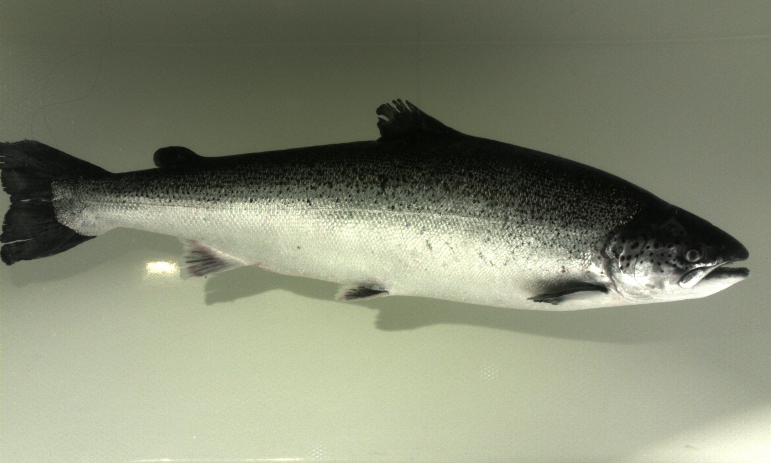
\includegraphics[width=.99\linewidth]{images/literature/filtering/original_fish}
        \caption{Original Image}
    \end{subfigure}%
    \begin{subfigure}{.5\textwidth}
        \centering
        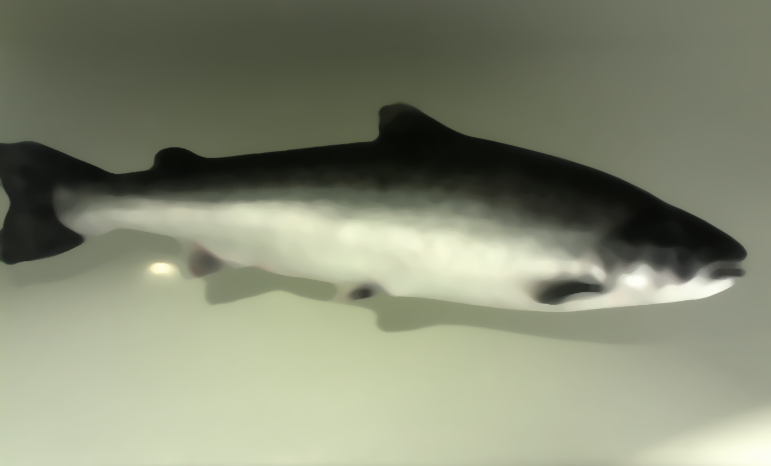
\includegraphics[width=.99\linewidth]{images/literature/filtering/median}
        \caption{Median Filter}
    \end{subfigure}
    \caption{Example of Median Filtering}
    \label{fig:median_filter}
\end{figure}

It is seen from the images in figure \ref{fig:median_filter} that both the background and all patterns on the fish are smoothed out, while the edges are preserved. Small particles is also removed; for example it is possible to see that some of the white reflections on the bottom of the image are gone and that all the black spots on the fish are blurred out. 
The median filter used on this image was filtered 2 times in a row. When filtering several times in a row instead of increasing the kernel size the image will not get as blurry while small particles are still removed.


\subsubsection{Bilateral Filter}
The bilateral filter is, just as the median filter, a nonlinear digital filter used to remove noise, while preserving sharp edges. Each pixel in an image is replaced by a weighted average of intensity values from neighboring pixels. The weight does not only depend on distance, but also on the radiometric differences such as color intensity and depth distance.\cite{book:digital_image_processing}\cite{website:wiki_bilateral_filter}\cite{book:machine_vision}

\begin{figure}[ht]
    \centering
    \begin{subfigure}{0.5\textwidth}
        \centering
        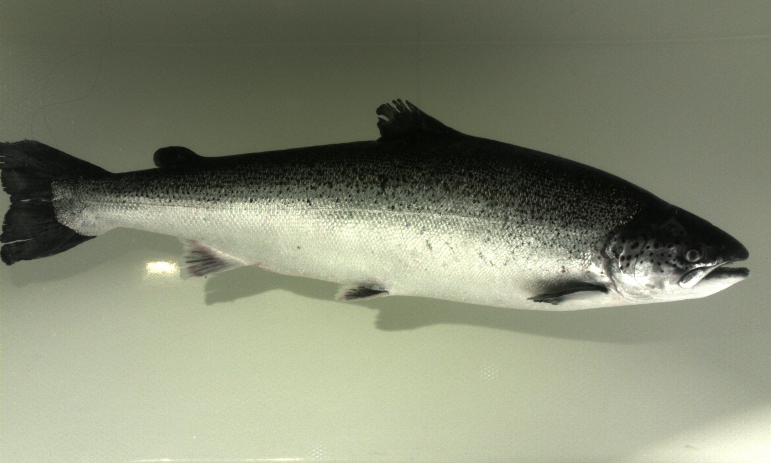
\includegraphics[width=.99\linewidth]{images/literature/filtering/original_fish}
        \caption{Original Image}
    \end{subfigure}%
    \begin{subfigure}{.5\textwidth}
        \centering
        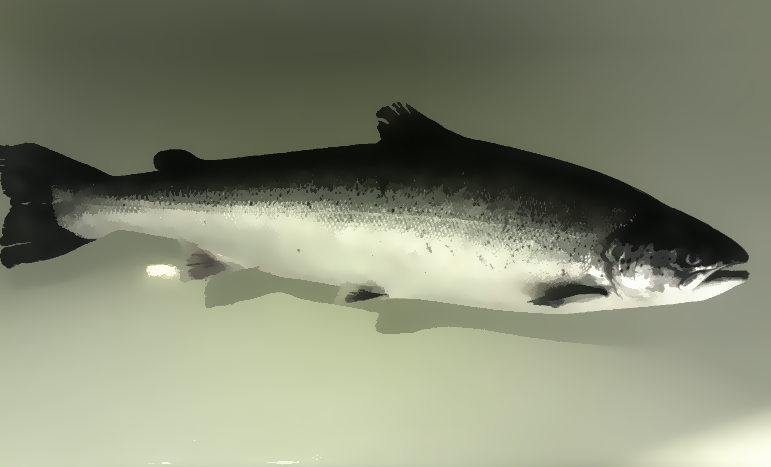
\includegraphics[width=.99\linewidth]{images/literature/filtering/bilateral}
        \caption{Bilateral Filter}
        \label{fig:bilateral_filter_b}
    \end{subfigure}
    \caption{Example of Bilateral Filtering}
    \label{fig:bilateral_filter}
\end{figure}

From figure \ref{fig:bilateral_filter} it is possible to see that the edges and most detail on the fish are well preserved while small imperfections are blurred out. This filter also increases the intensity of the image. This image was also filtered several times in a row instead of using a larger kernel size.


%%%%%%%%%%%%%%%%%%%%%%%%%%%%%%%%%%%%%%%%%%%%%%%%%%%%%%%%%%%%%%%%%%%%%%


\subsection{Filtering in the Frequency Domain}

The frequency domain is a space in which the image value at some pixel represents the amount that the intensity values vary over some distance. Changes done in the frequency domain affects the rate at which the intensity values are changing in the spatial domain.\cite{website:frequency_domain}
The Fourier Transform is mostly used to convert images from the spatial domain into the frequency domain, and the Inverse Fourier Transform is used to convert the other way. 
Filtering in the frequency domain is mostly used for removing continuous patters that occur in the spatial domain image.
Filtering in the frequency domain is also faster than running an averaging filter in the spatial domain, especially as the kernel size increases.\cite{website:frequency_domain_2}\cite{book:digital_image_processing}

In the frequency domain the spectrum is used to see the amplitudes of the sinusoids. A large amplitude implies a pattern in the spatial image. By removing the wanted amplitudes from the spectrum and using the Inverse Fourier Transform, the pattern formed from the amplitudes will be removed.
By removing certain frequencies in the frequency domain it is possible to remove patters like stripes on old images. The 2D images generated by the Raytrix technology will also have some small patterns caused by the micro lenses. This pattern is visible almost as a hexagon pattern.
Figure \ref{fig:hexagon_pattern} shows one small part from a totalfocus image generated by the Raytrix with an overlay showing the visible hexagon pattern.

\begin{figure}[ht]
    \centering
    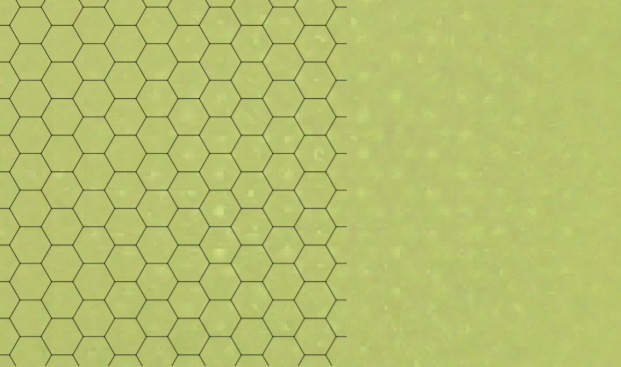
\includegraphics[width=0.7\textwidth]{images/literature/filtering/pattern_totalfocus}
    \caption{Pattern from Raytrix Totalfocus Image}
    \label{fig:hexagon_pattern}
\end{figure}

In many underwater images the light rays from either the sun or an external light source shows up as stripes in the image. If desired, these light rays could also be removed by filtering in the frequency domain. Section \ref{light_scattering} explains why these light rays occur in underwater images, and why objects appear blurry underwater.


%%%%%%%%%%%%%%%%%%%%%%%%%%%%%%%%%%%%%%%%%%%%%%%%%%%%%%%%%%%%%%%%%%%%%%


\subsection{Morphological Operators}

Morphology is a wide set of operations that process images based on shapes.\cite{website:mathworks_morphology} The operators apply a structuring element to an input image, and the value of each pixel in the output image is based on a comparison of the pixel with its neighbors. The structuring element is chosen by size and shape, and therefore determines the operations sensitivity towards different shapes.\cite{book:digital_image_processing}\cite{book:machine_vision}
The shape of the structuring element can be chosen as flat or non-flat. Examples of flat structuring elements are ellipse, cross or rectangle, as shown below. Non-flat structuring elements have different weighting on the neighboring pixels.

\noindent Examples of flat structuring elements with kernel size 5:

\noindent Ellipse: 
$\begin{bmatrix}
    0 & 0 & 1 & 0 & 0 \\
    1 & 1 & 1 & 1 & 1 \\
    1 & 1 & 1 & 1 & 1 \\
    1 & 1 & 1 & 1 & 1 \\
    0 & 0 & 1 & 0 & 0
\end{bmatrix}$ 
Cross: 
$\begin{bmatrix}
    0 & 0 & 1 & 0 & 0 \\
    0 & 0 & 1 & 0 & 0 \\
    1 & 1 & 1 & 1 & 1 \\
    0 & 0 & 1 & 0 & 0 \\
    0 & 0 & 1 & 0 & 0 
\end{bmatrix}$
Rect: 
$\begin{bmatrix}
    1 & 1 & 1 & 1 & 1 \\
    1 & 1 & 1 & 1 & 1 \\
    1 & 1 & 1 & 1 & 1 \\
    1 & 1 & 1 & 1 & 1 \\
    1 & 1 & 1 & 1 & 1
\end{bmatrix}$

\noindent Example of non-flat structuring element:
$\begin{bmatrix}
    0 & 0 & 1 & 0 & 0 \\
    0 & 1 & 2 & 1 & 0 \\
    1 & 2 & 4 & 2 & 1 \\
    0 & 1 & 2 & 1 & 0 \\
    0 & 0 & 1 & 0 & 0
\end{bmatrix}$ 

Morphological operators are useful for separating objects from each other, or merging objects together. It can also be used to remove small objects from an image, separate objects, merge objects, or highlight certain objects.


\subsubsection{Dilate and Erode}
The most basic morphological operators are dilation and erosion. These operators also make the base for all morphological operators. On gray-scale images dilation will add pixels on white object boundaries, while erosion will add pixels on black object boundaries. Dealing with multi-channel images, each channel is normally processed independently. Dilation and erosion is defined as follows:
\begin{itemize}
    \item Dilation: The value of the output pixel is the \textit{maximum} value of all pixels in the input pixels neighborhood.\cite{website:mathworks_morphology} 
    \item Erosion: The value of the output pixel is the \textit{minimum} value of all pixels in the input pixels neighborhood.\cite{website:mathworks_morphology}
\end{itemize}

Figure \ref{fig:star_dilate_erode} shows an example of dilation and erosion on a simple binary image, and figure \ref{fig:nemo} shows how dilation and erosion modifies a color image.

\begin{figure}[ht]
    \centering
    \begin{subfigure}{0.33\textwidth}
        \centering
        
\includegraphics[width=.99\linewidth]{images/literature/morphological/star}
        \caption{Original Image}
    \end{subfigure}%
    \begin{subfigure}{.33\textwidth}
        \centering
        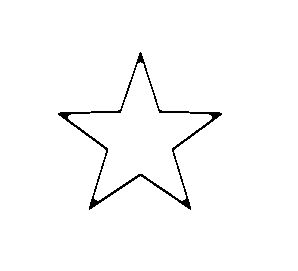
\includegraphics[width=.99\linewidth]{images/literature/morphological/dilation}
        \caption{Dilated}
    \end{subfigure}%
    \begin{subfigure}{.33\textwidth}
        \centering
        
\includegraphics[width=.99\linewidth]{images/literature/morphological/erosion}
        \caption{Eroded}
    \end{subfigure}
    \caption{Example of Dilation and Erosion}
    \label{fig:star_dilate_erode}
\end{figure}


\begin{figure}[ht]
    \centering
    \begin{subfigure}{0.33\textwidth}
        \centering
        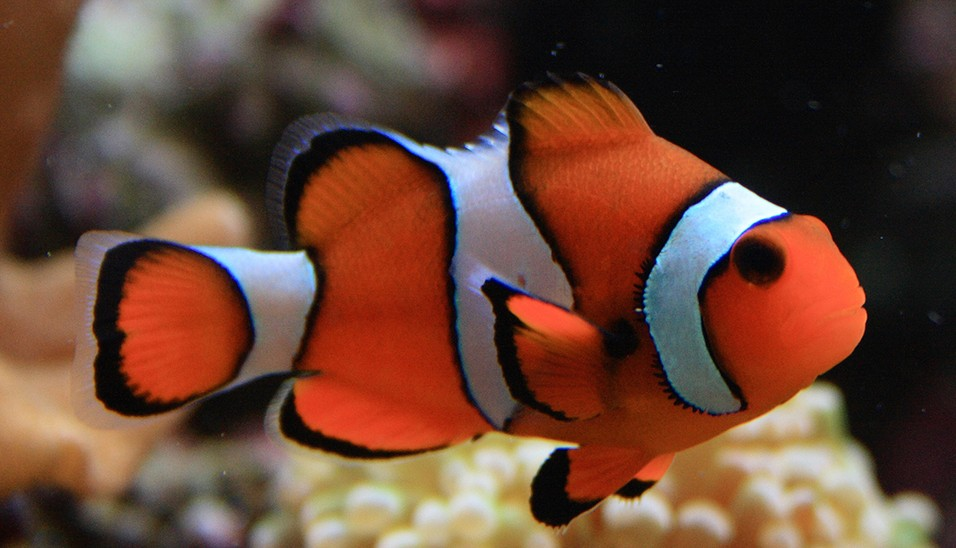
\includegraphics[width=.99\linewidth]{images/literature/morphological/nemo}
        \caption{Original Image\cite{website:klovnefisk_image}}
    \end{subfigure}%
    \begin{subfigure}{.33\textwidth}
        \centering
        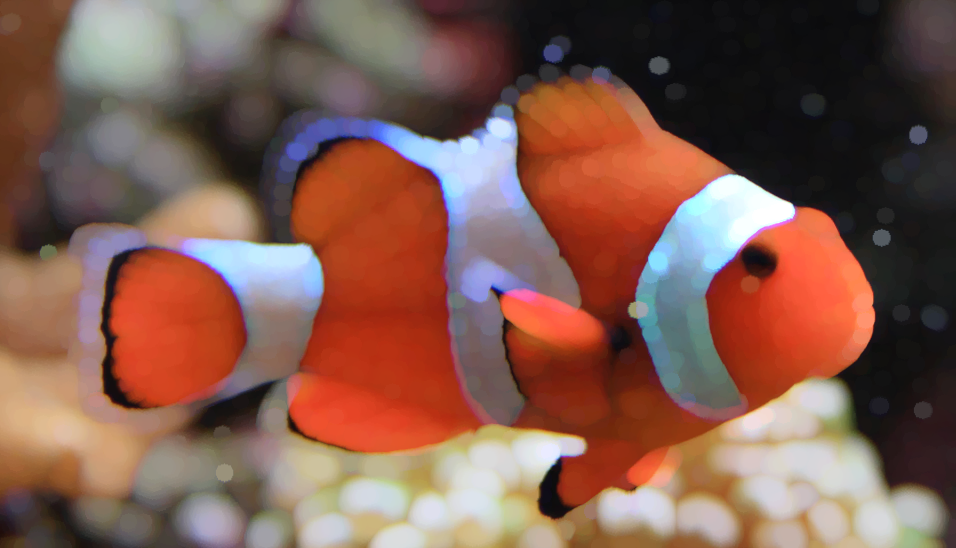
\includegraphics[width=.99\linewidth]{images/literature/morphological/nemo_dilate}
        \caption{Dilated}
    \end{subfigure}%
    \begin{subfigure}{.33\textwidth}
        \centering
        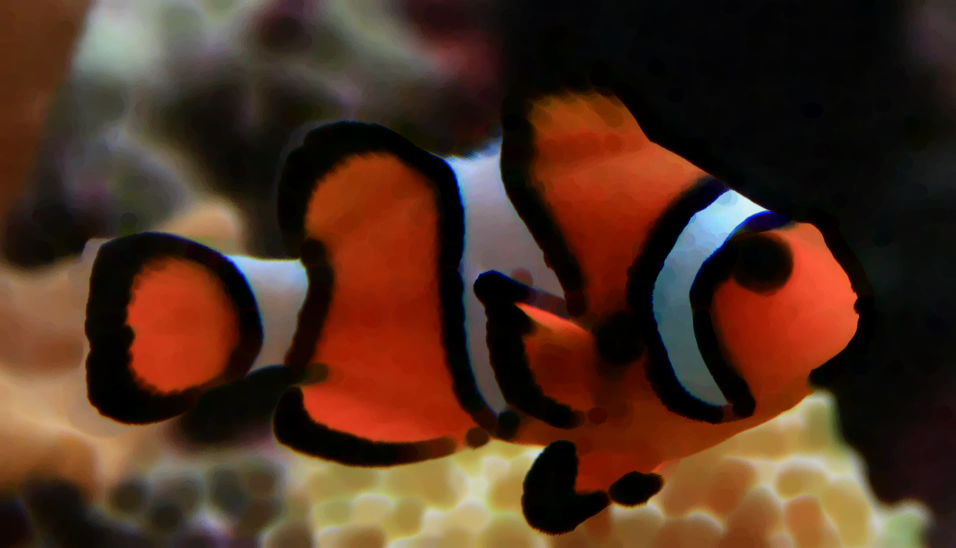
\includegraphics[width=.99\linewidth]{images/literature/morphological/nemo_erode}
        \caption{Eroded}
    \end{subfigure}
    \caption{Example of Dilation and Erosion on Color Image}
    \label{fig:nemo}
\end{figure}



\subsubsection{Opening and Closing}
Opening and closing are combinations of dilation and erosion. Opening is the dilation of the erosion of an image, while closing is the erosion of the dilation of an image. 

\begin{figure}[ht]
    \centering
    \begin{subfigure}{0.33\textwidth}
        \centering
        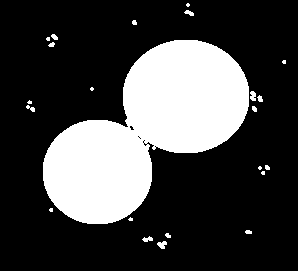
\includegraphics[width=.99\linewidth]{images/literature/morphological/dots}
        \caption{Original Image}
    \end{subfigure}%
    \begin{subfigure}{.33\textwidth}
        \centering
        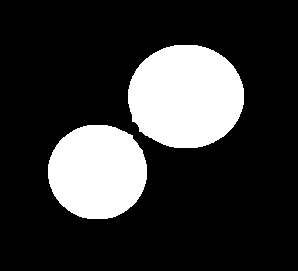
\includegraphics[width=.99\linewidth]{images/literature/morphological/opening}
        \caption{Opened}
    \end{subfigure}%
    \begin{subfigure}{.33\textwidth}
        \centering
        
\includegraphics[width=.99\linewidth]{images/literature/morphological/closing}
        \caption{Closed}
    \end{subfigure}
    \caption{Example of Opening and Closing}
    \label{fig:dots_opening_closing}
\end{figure}

Opening and closing assumes bright objects on a dark background. When opening an image, small objects will be removed and objects close to each other will be separated. When closing an image, objects close to each other will be closed together into one object. See figure \ref{fig:dots_opening_closing}.


%%%%%%%%%%%%%%%%%%%%%%%%%%%%%%%%%%%%%%%%%%%%%%%%%%%%%%%%%%%%%%%%%%%%%%


\subsection{Thresholding}

Thresholding is a simple image segmentation method. It is mostly used on grayscale images to obtain a binary image. In its simples form it replaces each pixel with black if the the intensity is less than some fixed threshold value, and with white if the intensity is above the threshold value. This form of thresholding is called global thresholding.\cite{website:thresholding}\cite{website:wiki_threshold}
The threshold value can be set manually, or chosen by the computer, depending on the threshold method used. 

Thresholding is mostly used to detect brighter objects from the darker background background, or opposite, detect darker objects from the lighter background.
From this, it is easy to understand that the global thresholding method is not optimal for images where the background color varies between being darker and brighter than the object.
Luckily, for solving problems like this, more advanced thresholding methods do exist.


\subsubsection{Adaptive Thresholding}
Sometimes the intensity of both the object and the background changes rapidly throughout the image. This makes it hard to set a threshold value that holds for the entire image. In these situations local thresholding is the solution. Local (adaptive) thresholding runs through each pixel and chooses a threshold value based on each pixel's neighborhood. How the threshold value for each pixel is chosen is for the user to decide, but most common is the median value or the Gaussian mean value of the neighborhood.

Deciding which method to use depends all on the type of image. With clear differences between the object and the background, global thresholding is preferred. If the background color varies, or if the object detected is a contour, lines or text, adaptive threshold performs better.
\newline

Figure \ref{fig:fish_threshold} shows an example of both global and adaptive thresholding. If the task is to detect the whole fish, and the fish only, it is clear to see that global thresholding performs better than adaptive thresholding. If the task was to get the contour of the object, adaptive thresholding would be better. 

Figure \ref{fig:text_threshold} shows an example of a grayscale image of text that should be converted to binary while containing the text. Since the colors varies, global thresholding does not perform well here, while adaptive thresholding gives good results.


\begin{figure}[H]
    \centering
    \begin{subfigure}{0.33\textwidth}
        \centering
        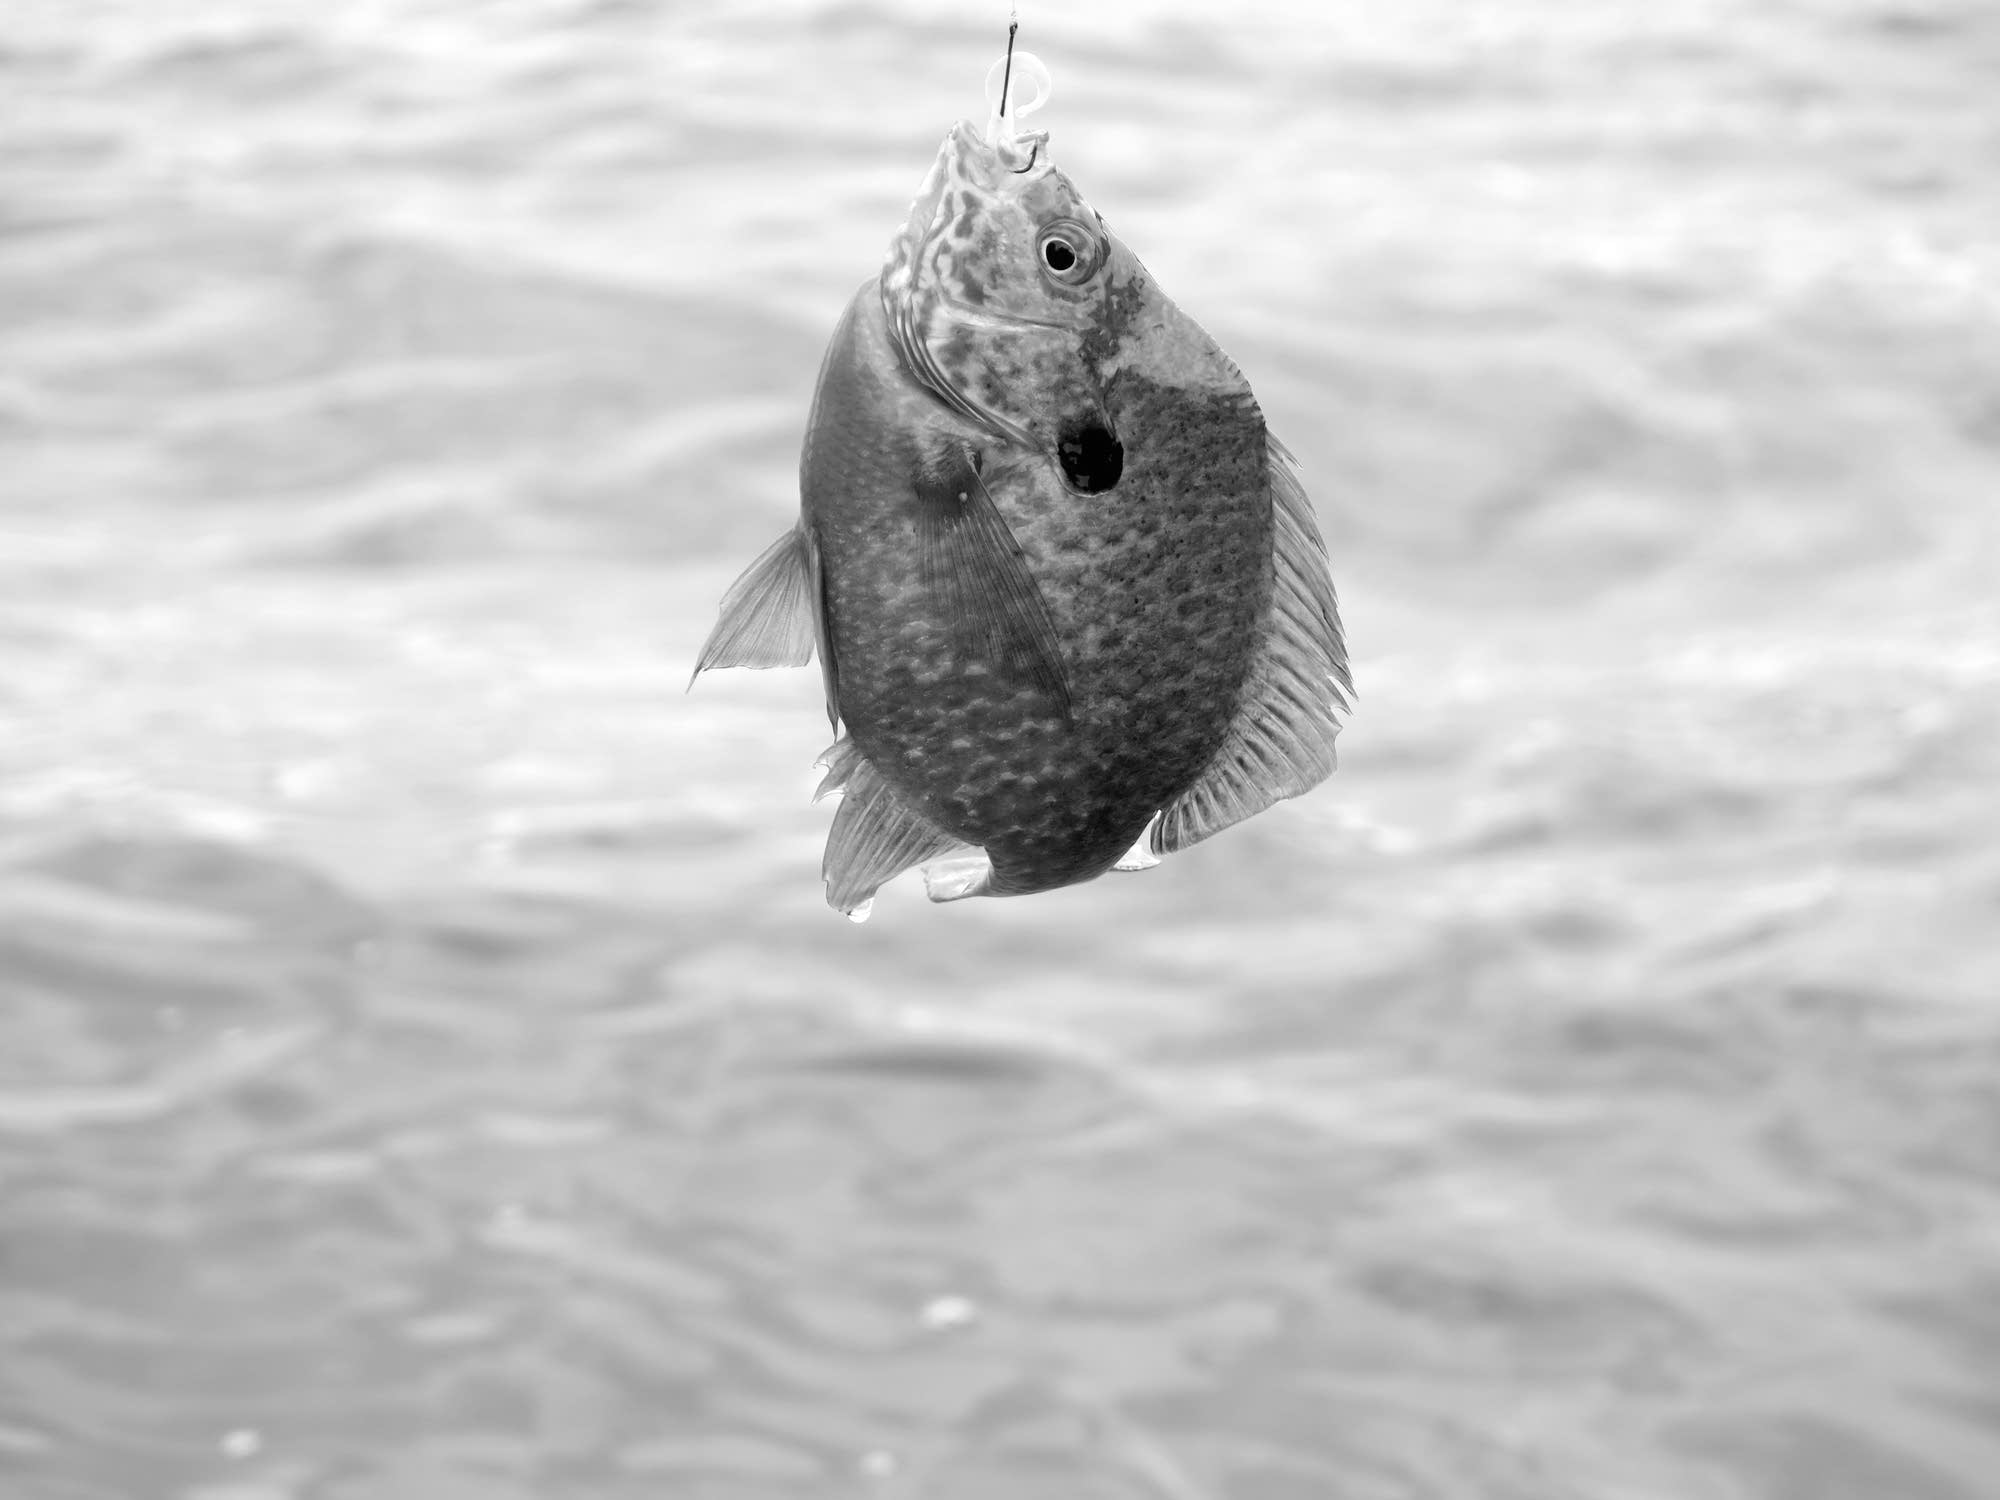
\includegraphics[width=.99\linewidth]{images/literature/thresholding/original_fish_grayscale}
        \caption{Original Image\cite{website:colorfish_image}}
    \end{subfigure}%
    \begin{subfigure}{.33\textwidth}
        \centering
        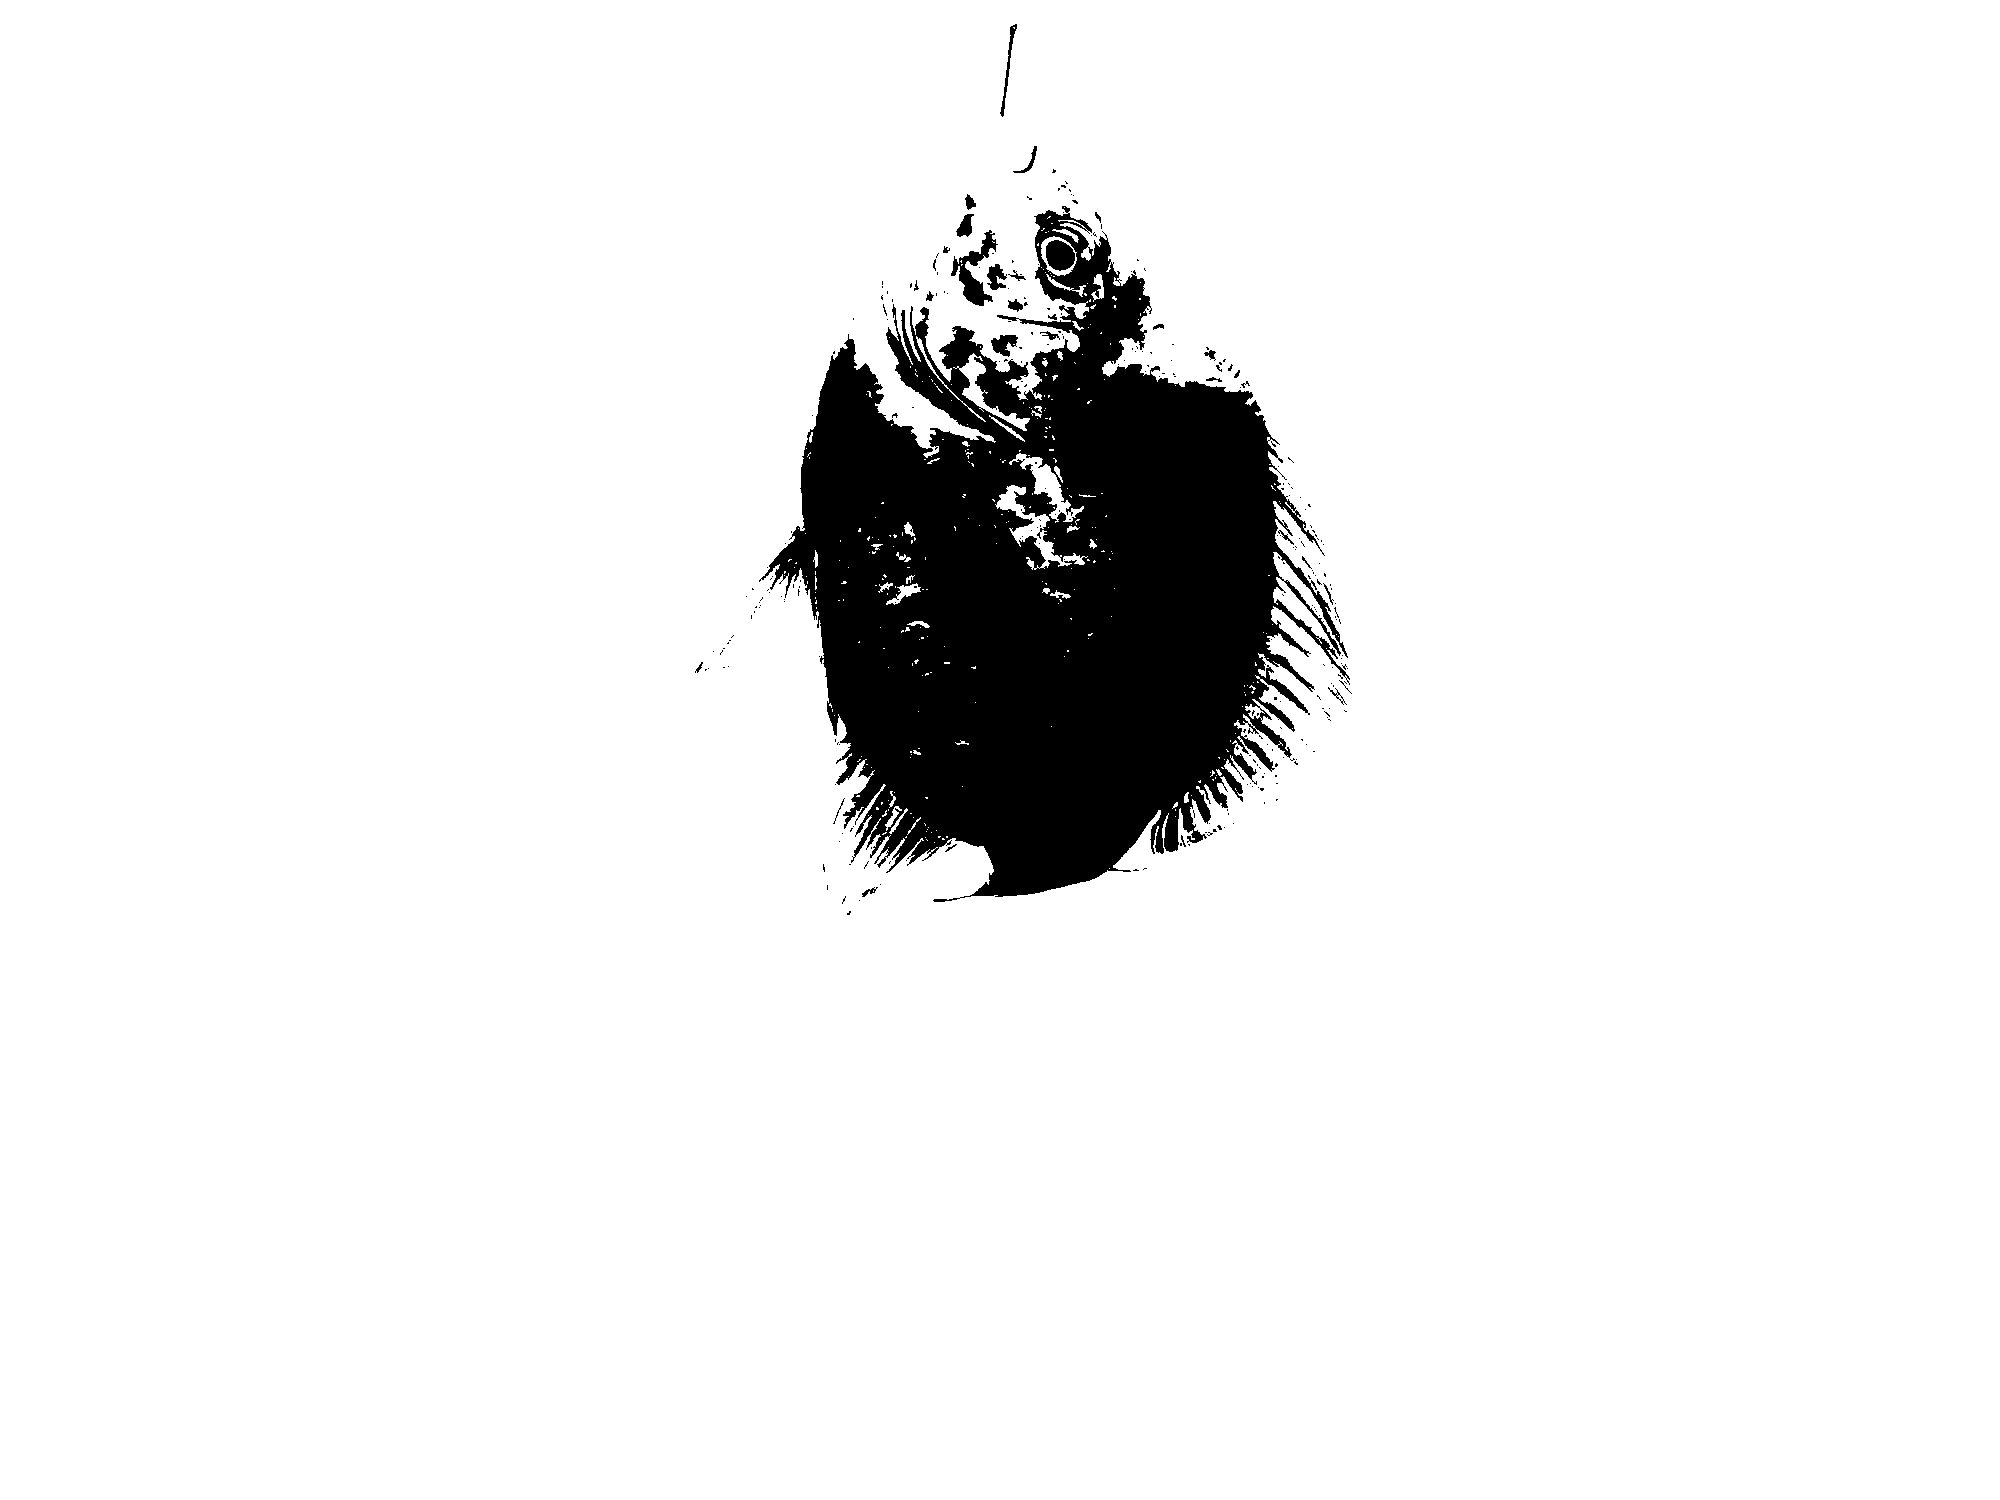
\includegraphics[width=.99\linewidth]{images/literature/thresholding/fish_global_thresholding}
        \caption{Global Thresholding}
    \end{subfigure}%
    \begin{subfigure}{.33\textwidth}
        \centering
        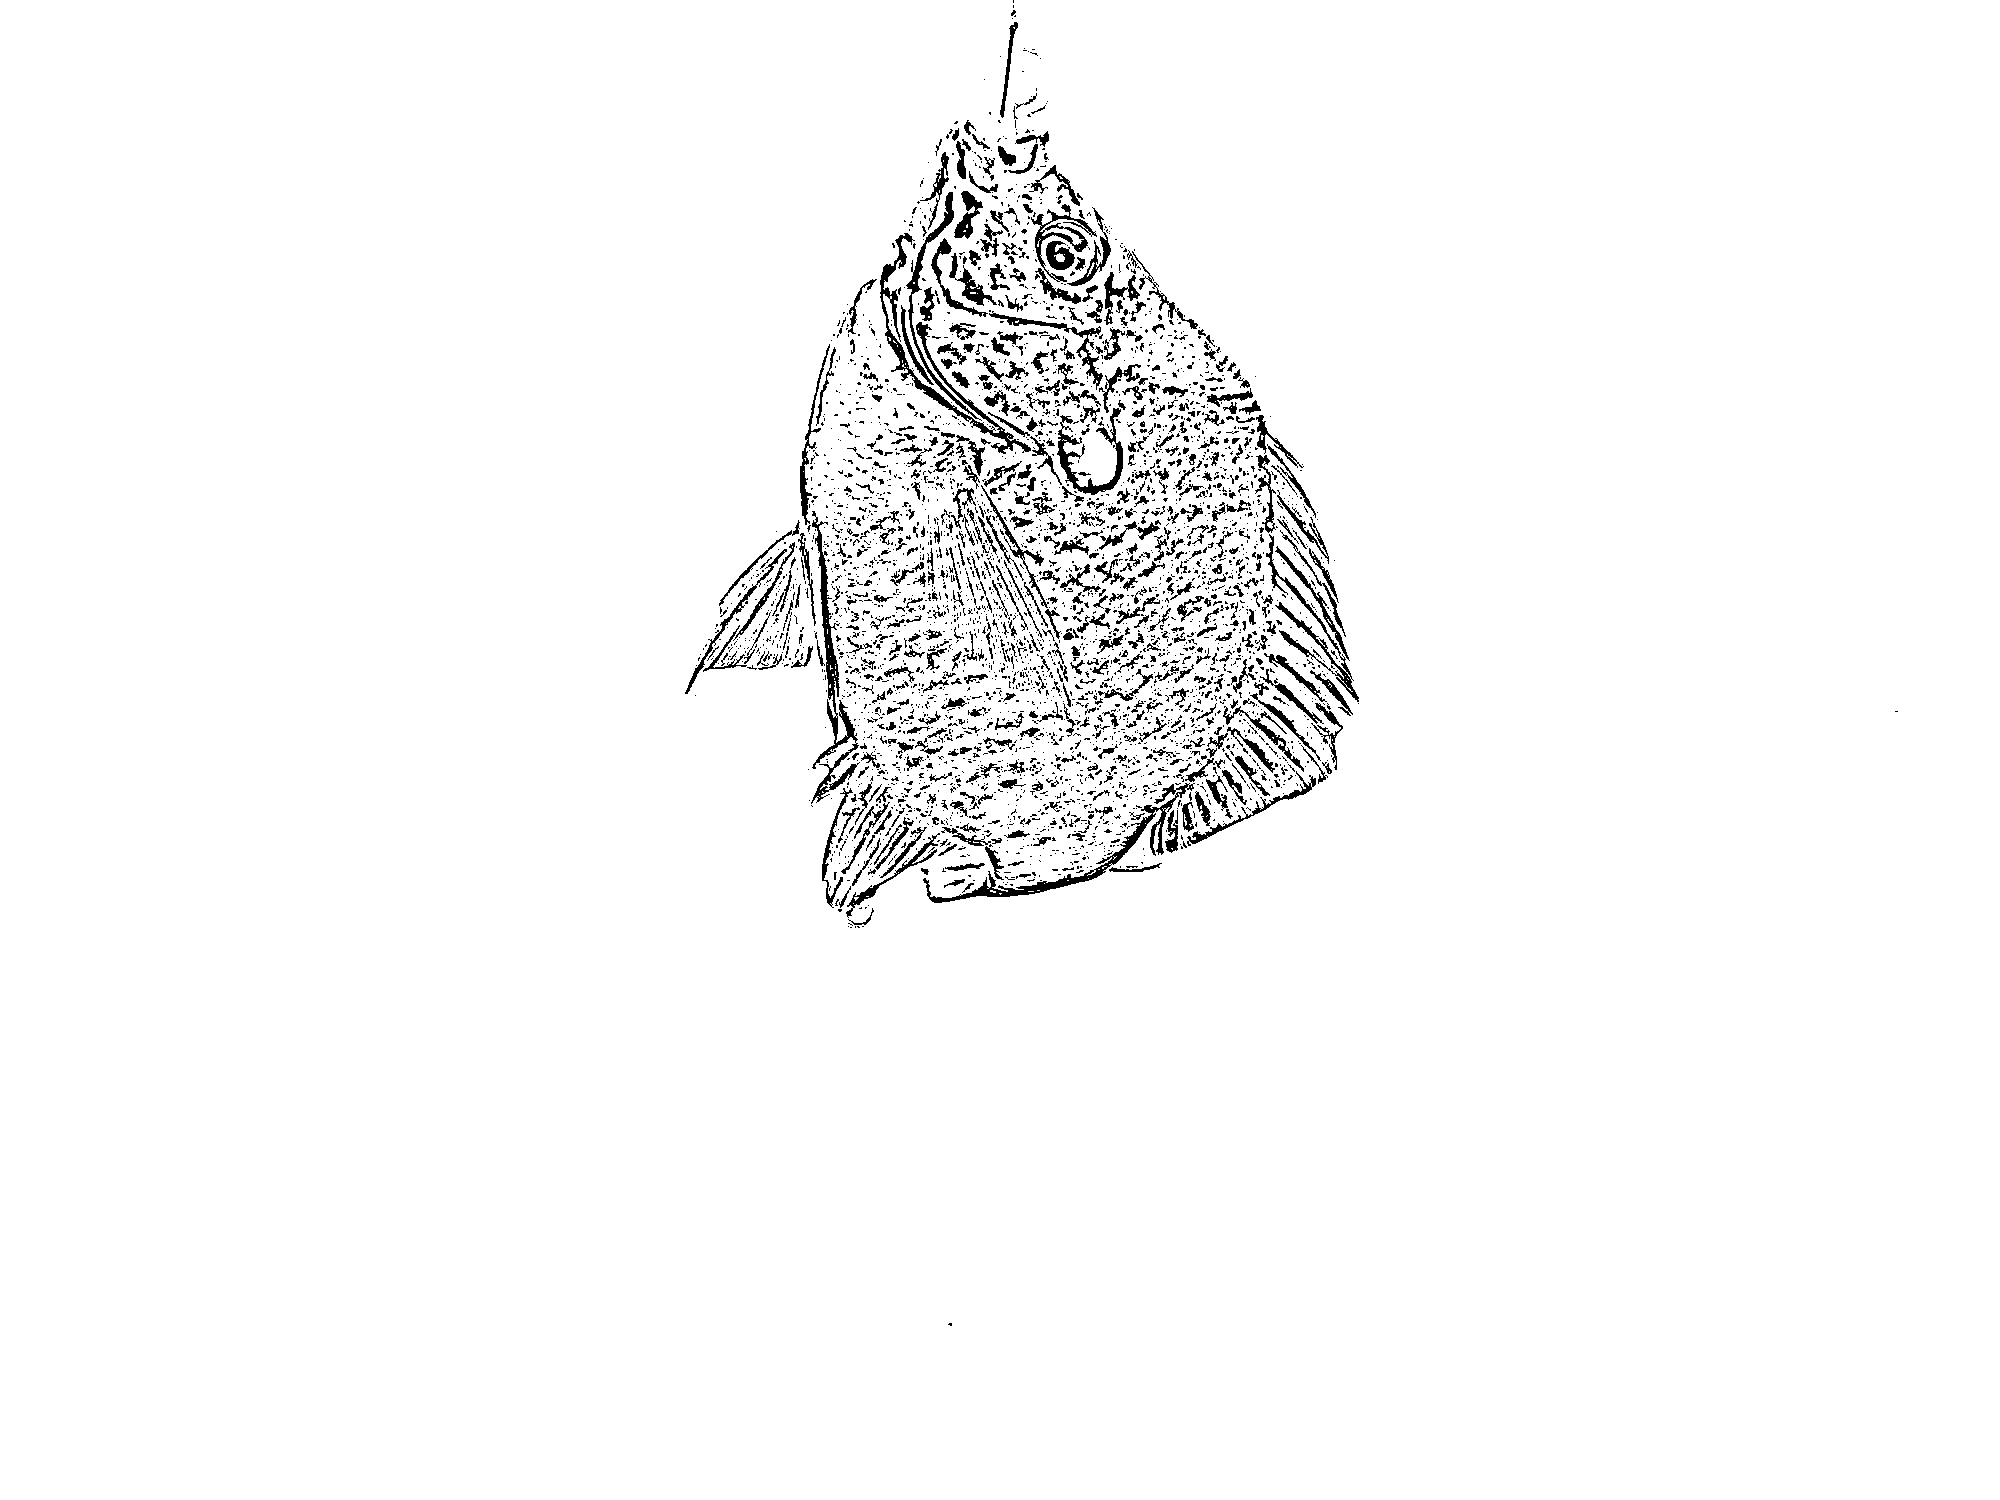
\includegraphics[width=.99\linewidth]{images/literature/thresholding/fish_adaptive_thresholding}
        \caption{Adaptive Thresholding}
    \end{subfigure}
    \caption{Thresholding of Fish}
    \label{fig:fish_threshold}
\end{figure}


\begin{figure}[H]
    \centering
    \begin{subfigure}{0.33\textwidth}
        \centering
        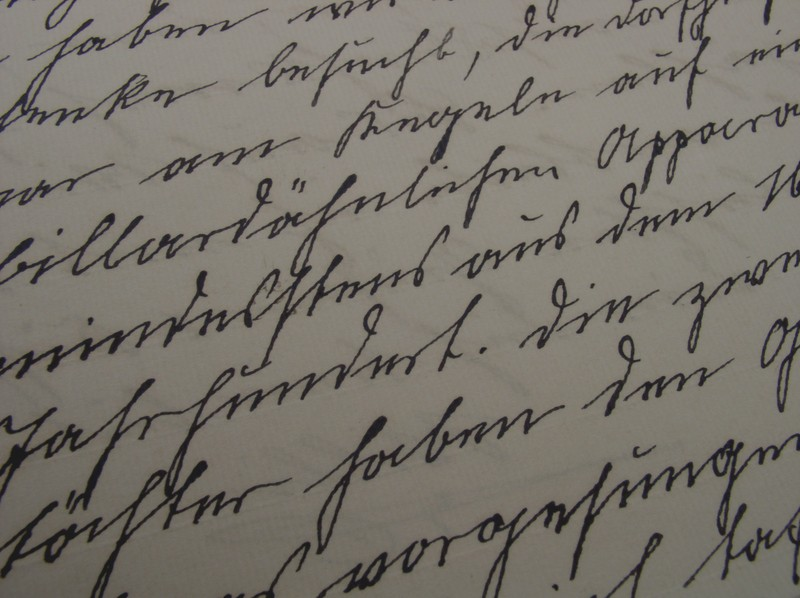
\includegraphics[width=.99\linewidth]{images/literature/thresholding/original_text}
        \caption{Original Image\cite{website:handwriting_image}}
    \end{subfigure}%
    \begin{subfigure}{.33\textwidth}
        \centering
        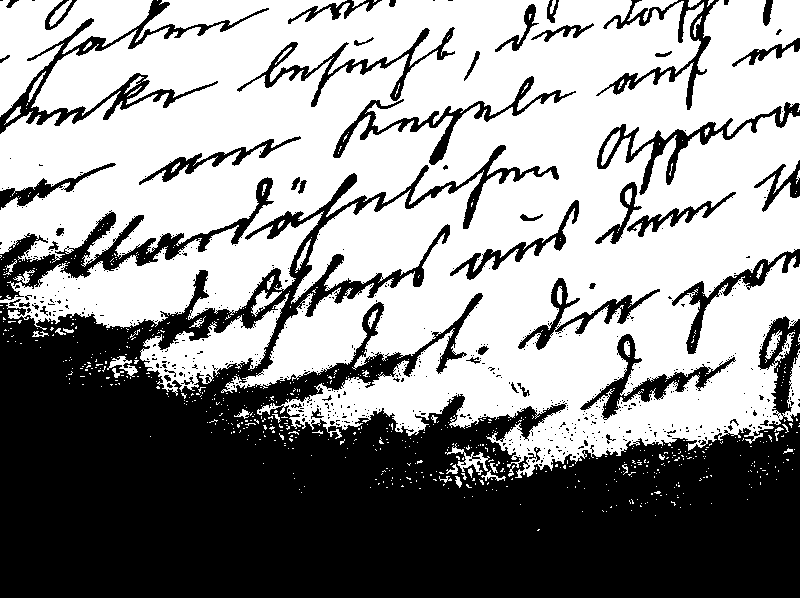
\includegraphics[width=.99\linewidth]{images/literature/thresholding/text_global_thresholding}
        \caption{Global Thresholding}
    \end{subfigure}%
    \begin{subfigure}{.33\textwidth}
        \centering
        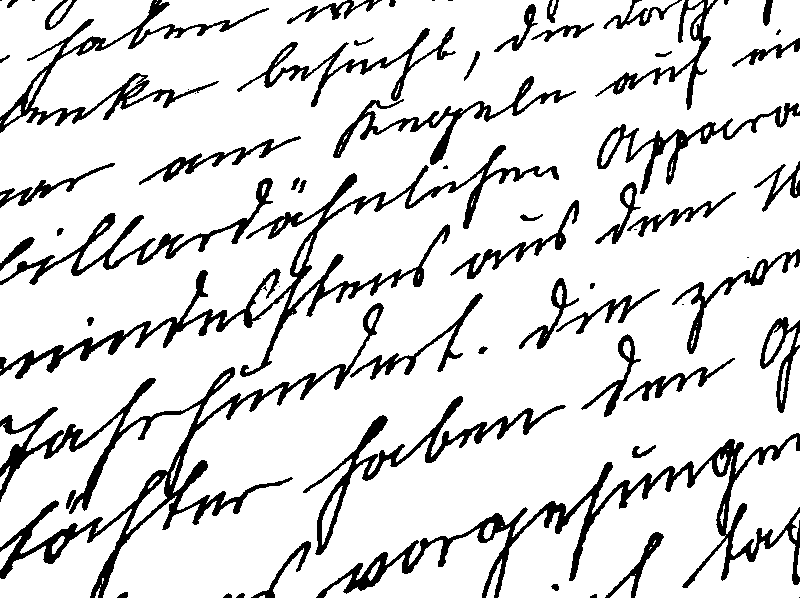
\includegraphics[width=.99\linewidth]{images/literature/thresholding/text_adaptive_thresholding}
        \caption{Adaptive Thresholding}
    \end{subfigure}
    \caption{Thresholding of Document}
    \label{fig:text_threshold}
\end{figure}


%%%%%%%%%%%%%%%%%%%%%%%%%%%%%%%%%%%%%%%%%%%%%%%%%%%%%%%%%%%%%%%%%%%%%%


\subsection{Light Scattering} \label{light_scattering}

Most objects that one sees are visible due to light scattering from their surfaces. Indeed, this is the primary mechanism of physical observation. Scattering of light depends on the wavelength or frequency of the light being scattered, so particles smaller than the wavelength is impossible to observe.\cite{website:wiki_light_scattering}

The light propagation in the water medium causes the observed objects to appear unclear or blurry. The physical properties of water cause degradation effects not present in air. The water absorbs light and therefore limits the visibility distance, while also causing scattering, which changes the direction of the light path. Underwater light scattering is the deflection of a ray from a straight path, caused by the irregularities in the water medium and particles. Deviations due to irregularities on the water surface are also usually considered as a form of scattering. 

This influences the overall performance of underwater imaging systems. Forward scattering is the spreading of light from an object towards the camera, while backward scattering is the light reflected by the water towards the camera before it actually reaches an object. Backward scattering reduces the contrast of the image, and is seen as light rays in the image. Scattering comes not only from the water itself, but also from all particles in the water and from the water surface.\cite{article:underwater_image_processing}

\begin{figure}[ht]
    \centering
    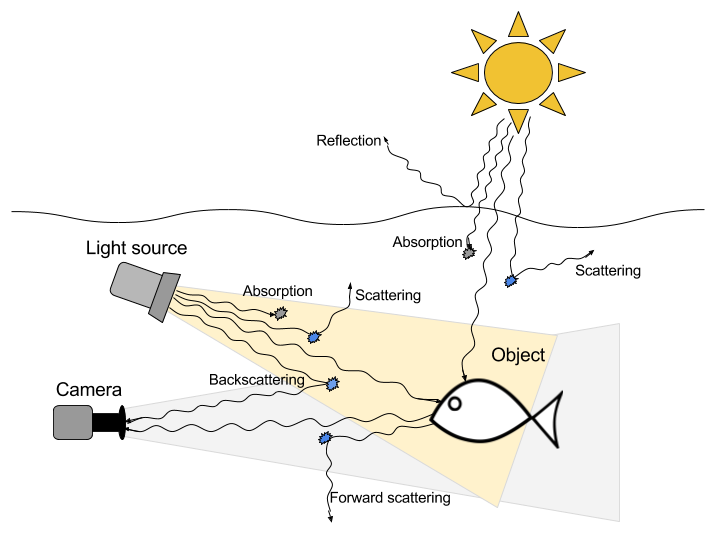
\includegraphics[width=0.99\textwidth]{images/literature/light_scattering}
    \caption{Explanation of Light Scattering in Water}
    \label{fig:light_scattering}
\end{figure}

